\documentclass{article}
\usepackage[utf8]{inputenc}
\usepackage{amsmath}
\usepackage{listings}
\usepackage{graphicx}
\usepackage{geometry}
\usepackage{float}

\usepackage[style=alphabetic,backend=biber,
bibencoding=utf8, natbib=true
]{biblatex}
\addbibresource{Quellen.bib}

\usepackage{color}
 
\definecolor{codegreen}{rgb}{0,0.6,0}
\definecolor{codegray}{rgb}{0.5,0.5,0.5}
\definecolor{codepurple}{rgb}{0.58,0,0.82}
\definecolor{backcolour}{rgb}{0.95,0.95,0.92}
 
\lstdefinestyle{mystyle}{
    backgroundcolor=\color{backcolour},   
    commentstyle=\color{codegreen},
    keywordstyle=\color{magenta},
    numberstyle=\tiny\color{codegray},
    stringstyle=\color{codepurple},
    basicstyle=\footnotesize,
    breakatwhitespace=false,         
    breaklines=true,                 
    captionpos=b,                    
    keepspaces=true,                 
    numbers=left,                    
    numbersep=5pt,                  
    showspaces=false,                
    showstringspaces=false,
    showtabs=false,                  
    tabsize=2
}
\geometry{a4paper,left=30mm,right=30mm, top=3cm, bottom=3cm}

\lstset{style=mystyle}
\begin{document}
\begin{titlepage}


\begin{figure}[H]
  \begin{minipage}[t]{.49\textwidth}
    \includegraphics[width=.8\textwidth]{hu-logo.png}  
  \end{minipage}
  \label{fig:spektren01sd}
\end{figure}

\vspace{10mm}


\begin{center}
		\vspace{2cm}
		{\huge\bfseries Portfolio Optimization Strategies \par}
		\vspace{2cm}
		{\scshape\LARGE Iliyana Pekova and Georg Velev\par}
		\vspace{2cm}
		{\huge\large March 2019 \par}
		
\end{center}
\end{titlepage}

\tableofcontents
\vspace{3cm}
\medskip
Link to GitHUb-Quantlet: \url{https://github.com/pekova13/SPL_MeanVar_ThreeFund.git}
\section{Introduction}
Portfolio optimization refers to choosing the best portfolio that consists of particular assets according to certain evaluation criteria. In this context, optimization strategies in the field of finance are applied in order to compute the optimal set of relative weights of the assets available for investment. These weights in turn determine the structure of the optimal portfolio by predefining how much should be invested in each of these assets.\endgraf
The aim of this research is to implement two of the portfolio strategies described by DeMiguel et al. \cite{DEM09}, the mean-variance strategy and the three-fund one, and to evaluate their performance in-sample as well as out-of-sample. Hence, this research replicates the methodology applied by DeMiguel et al. \cite{DEM09} and compares the yielded results. The "S \& P Sectors" dataset which is created by Roberto Wessels is used for this purpose. It is composed by 10 value-weighted industry portfolios and the S\&P 500 index which is used as the benchmark portfolio. The time window is set from January 1981 to December 2002.\endgraf
This report consists of four sections. First, the theoretical background of the chosen portfolio strategies and of the opted for evaluation criteria is described. Then, Section 3 presents the strategy-dependent as well as the strategy-independent functions applied. Afterward, the results of the empirical research are reported and certain visualization tools are used in order to present some patterns in the data. The last section provides a short summary.

\section{Theory}
\subsection{Evaluation Metrics}
\subsubsection{Sharpe Ratio}
The first evaluation metric is the sharpe ratio. It is defined as the additional excess return an investor receives for the extra risk (expressed in volatility) they take by holding a risky asset/portfolio \cite{SHP}. DeMiguel et al. \cite{DEM09} suggest two approaches for the calculation of the sharpe ratio: in-sample and out-of-sample.\endgraf
The in-sample alternative computes a single relative weights vector based on the data from the complete observation period. The asset excess returns for each period are then weighted by this vector. The end result is a vector of in-sample portfolio returns. The mathematical in-sample sharpe ratio formula looks as follows \cite{DEM09}:
\begin{align}
\hat{SR}_{k}^{IS} = \frac{Mean_{k}}{\splitfrac{Std_{k}}} = \frac{\hat{\mu}_{k}^{IS}\hat{w}_{k}}{\splitfrac{\sqrt{\hat{w}_{k}^{T}\hat{\Sigma}_{k}^{IS}\hat{w}_{k}}}}
\end{align}
where $\hat{\mu}_{k}^{IS}$ is the estimated means vector of all assets for the whole period of observation for investment strategy $k$, $\hat{w}_{k}$ the estimated in-sample relative weights vector for strategy $k$ and $\hat{\Sigma}_{k}^{IS}$ the estimated in-sample co-variance matrix for strategy $k$.\endgraf
The out-of-sample approach sets a rolling window of M periods. The relative weights vector for each period t starting from M+1 is then calculated based on the previous M observations and applied to the asset returns in the corresponding period t. The end result is a vector of length T-M containing the out-of-sample portfolio returns. The computation formula is the following \cite{DEM09}:
\begin{align}
\hat{SR}_{k} = \frac{\hat{\mu}_{k}}{\splitfrac{\hat{\sigma}_{k}}} 
\end{align} 
where $\hat{\mu}_{k}$ is the estimated mean of the out-of-sample portfolio returns for strategy $k$ and $\hat{\sigma}_{k}$ is the estimated standard deviation (a metric for risk/volatility) of the the out-of-sample portfolio returns for strategy $k$.
\subsubsection{Certainty-Equivalent}
The second evaluation metric is the certainty equivalent, which is defined as the guaranteed return an investor would accept now rather than taking the risk of a higher, but an uncertain return in the future \cite{CTA}. The certainty equivalent can also be computed in-sample (in-sample portfolio returns needed) and out-of-sample (out-of-sample portfolio returns needed). Both are calculated according to the following formula:
\begin{align}
\hat{CEQ}_{k} = \hat{\mu}_{k} - \frac{\gamma}{\splitfrac{2}}\hat{\sigma}_{k}^{2}
\end{align} 
where $\hat{\mu}_{k}$ is the estimated means of the portfolio returns for strategy $k$, $\gamma$ is the risk aversion, which in this particular case is set to 1 and $\hat{\sigma}_{k}^{2}$ is the estimated variance for the portfolio returns for strategy {k}. 
\subsection{Sample-based Mean-Variance-Portfolio}
\subsubsection{Qualitative Background}
The mean-variance portfolio optimization strategy is some of the most frequently used techniques to find the optimal set of relative weights for the construction of investment portfolios. The Markowitz portfolio theory provides investors with a model that achieves an optimal trade-off between the expected returns and the volatility. In addition to that, the standard deviation of the portfolio returns measures the total risk of a particular investment . Thus, the preferences of investors applying this optimization technique are entirely defined by the mean and the variance of the portfolio returns \cite{RAM07}.
\subsubsection{Quantitative Background}
Expressed in mathematical terms, this implies maximizing the objective function of the expected utility at time $t$ \cite{DEM09}:\\
\begin{align}
\max_{X_t} \ \ x^T_t\mu_t - \frac{\gamma}{\splitfrac{2}} x^T_t \Sigma\nolimits_{t}x_t ,
\end{align}\\
where $x_t$ is the chosen portfolio, $\mu_t$ is the vector of the expected returns on the risky assets in excess on the risk-free rate, $\gamma$ is the risk aversion of the investor and $\Sigma\nolimits_{t}$ is the co-variance matrix of the excess returns. Resolving the above equation results in the following vector of absolute weights for the optimal portfolio at time $t$:\\
\begin{align}
\ x_t =\frac{1}{\splitfrac{\gamma}}\Sigma\nolimits_{t}^{-1}\mu_t ,
\end{align}\\
where $\Sigma\nolimits_{t}^{-1}$ is the inverse of the co-variance matrix. In addition to that, the vector of relative weights at time $t$ can be defined as follows when $\gamma$ = 1:\\
\begin{align}
w_t = \frac{x_t}{\splitfrac{| 1_Nx_t |}} , 
\end{align}\\
where $N$ is the amount of risky assets being considered and $1_N$ is a N-dimensional vector of ones. In this context, $1_Nx_t$ represents the sum of the average excess returns. It is essential to underline, that the absolute value of the sum in the denominator ensures that any negative values in $x_t$ will not have an impact on the sign of the respective relative weights.
\subsubsection{Limitations}
The main limitation of the mean-variance strategy is related to the assumption that investors only consider the mean and the variance for the optimization of their portfolios. Hence, further potentially relevant measures of risk, for instance the downside risk, are not taken into account. Moreover, the Markowitz model is often criticized for completely ignoring the estimation error whenever the sample mean and the sample co-variance matrix are used as the estimates of the two moments of the return distributions, $\hat{\Sigma}$ and $\hat{\mu}$. In case the number of assets available for investment is large in relation to the number of the historical instances, the computation of the relative weights based on the  sample moments may yield imprecise results. 
\subsection{The Kan and Zhou Three-Fund Portfolio}
\subsubsection{Qualitative Background}
The Kan and Zhou three-fund portfolio investment strategy aims at the minimization of the estimation error, which results from the investor only holding the tangency portfolio and a risk-free asset. If the model parameters which maximize the utility function of the investor were known, their estimation would not be necessary and the risk of an estimation error would not exist. The investors would invest in the tangency portfolio and a risk-free asset without having to take the potential risks of uncertainty. However, since neither the true model parameters are directly observable, nor the exact utility function of the investor is known, the model parameters must be estimated and therefore an estimation error is practically inevitable. Thus, Kan and Zhou\cite{RAM07} suggest an approach which extends the investor's funds by an additional risky portfolio with the purpose of minimizing the estimation error. This idea is based on the assumption that the estimation errors of both risky portfolios are not perfectly correlated, which in turn diversifies the risk of the tangency portfolio. Hence, the goal of the three-fund portfolio strategy is to determine the relative weights of the assets held in the second risky portfolio (= the third fund). 
\subsubsection{Quantitative Background}
The relative weights of the second risky portfolio are computed according to the following rule:\\
\begin{align}
\hat{w} = \hat{w}(c,d) = \frac{1}{\splitfrac{\gamma}}(c\hat{\Sigma}^{-1}\hat{\mu} +
d\hat{\Sigma}^{-1}1_{N})   
\end{align}\\
The parameters c and d are the ones which lead to the optimal relative asset weights, meaning the ones which maximize the investor's utility. Like in the mean-variance strategy the parameter $\hat{\Sigma}^{-1}$ is the co-variance matrix of the adjusted asset returns and $\hat{\mu}$ is the means vector. According to Kan and Zhou the optimal values of c and d are the following ones:\\
\begin{align}
c^{**} = c_{3}\bigg(\frac{\psi^{2}}{\splitfrac{\psi^{2} + \frac{N}{\splitfrac{T}}}}\bigg) \\
d^{**} = c_{3}\bigg(\frac{\frac{N}{\splitfrac{T}}}{\splitfrac{\psi^{2} + \frac{N}{\splitfrac{T}}}}\bigg)\mu_{g} 
\end{align}\\
where N is the amount of the assets to be considered (including the benchmark asset) and T is the total amount of observations. The computation of $c_{3}$, $\mu_{g}$ and $\psi^{2}$ is based on the following formulas:\\
\begin{align}
c_{3} = \frac{(T-N-1)(T-N-4)}{\splitfrac{T(T-2)}} \\
\psi^{2} = (\mu - \mu_{g}1_{N})^{'}\hat{\Sigma}^{-1}(\mu - \mu_{g}1_{N})\\
\mu_{g} = \frac{(\hat{\mu}^{'}\hat{\Sigma}^{-1}1_{N})}{\splitfrac{(1^{'}_{N}\hat{\Sigma}^{-1}1_{N})}}  
\end{align}\\
where $\psi^{2}$ is the squared slope of the asymptote to the ex-ante minimum-variance frontier and $\mu_{g}$ is the expected excess return of the ex-ante global minimum-variance portfolio. After substituting (8) and (9) in (7), the absolute weights vector looks as follows:\\

\begin{align}
\hat{w}^{**} = \frac{c_{3}}{\splitfrac{\gamma}}\bigg[\bigg(\frac{\psi^{2}}{\splitfrac{\psi^{2}+\frac{N}{\splitfrac{T}}}}\bigg)\hat{\Sigma}^{-1}\hat{\mu} + \bigg(\frac{\frac{N}{\splitfrac{T}}}{\splitfrac{\psi^{2}+\frac{N}{\splitfrac{T}}}}\bigg)\mu_{g}\hat{\Sigma}^{-1}1_{N}\bigg]   
\end{align}

The relative weights vector is then computed as described in section 2.2.2 equation 6).

\section{Implementation}
\subsection{Strategy-independent Functions}
\subsubsection{Relative Weights Vector}
\begin{lstlisting}[caption={This example shows how relative weights vector is computed in R.}, label=code:1, frame = single]
get_rel_weights_vector = function(weights_vector){
    abs_sum = abs(sum(weights_vector))
    rel_weights = weights_vector/abs_sum
    return (rel_weights)
}
\end{lstlisting}
The computation of the relative weights vector does not directly depend on the applied financial strategy. The only parameter the function requires is the absolute weights vector, whose computation is strategy-dependent. As shown in the 4th line, firstly the total sum of the absolute weights must be built. Then the relative weights vector is calculated by dividing each value of the absolute weights vector by the total sum (7th line)  

\subsubsection{In-Sample Sharpe Ratio}
\begin{lstlisting}[caption={This example shows how the in-sample sharpe ratio and the in-sample portfolio returns are computed in R.}, label=code:1, frame=single]
get_insample_sharperatio_returns = function (data, absolute_weights_vector, sharperatio){
  
  pf_rtr_in_sample = c(length = length(data[,1]))
  for(i in 1:(length(data[,1]))){
    pf_rtr_in_sample[i] = unlist(data[i,])%*%(get_rel_weights_vector(absolute_weights_vector))
  }
  
  if (sharperatio == TRUE) {
    return (mean(pf_rtr_in_sample)/sd(pf_rtr_in_sample)) 
  } else { 
    return (pf_rtr_in_sample)
  }
}
\end{lstlisting}
The computation is based on formula (1). The function is designed to return either the in-sample sharpe ratio or a vector of the portfolio returns (result of weighting the single assets' returns with the computed relative weights for each period) over all considered time periods. The function was programmed this way in order to avoid code redundancies, since both the in-sample sharpe ratio and the portfolio returns vector have an essential piece of code in common (lines 3-6). The return is determined by the boolean parameter "sharperatio" in the 1st line. If the parameter is assigned "TRUE" the function returns the in-sample sharpe ratio, if assigned "FALSE" - the in-sample portfolio returns. The mutual code consists in creating an empty vector (line 3) and to fill it through a loop with the portfolio returns for each period (lines 4-6). The differentiation between both alternative return objects takes places in the 8th line by the use of an if-else construct. Line 9 returns the in-sample sharpe ratio after applying formula (1) on the in-sample portfolio returns vector resulting from the loop. Line 10 considers the case, in which the parameter sharperatio is assigned FALSE and thr function simply returns the portfolio returns vector.

\subsubsection{Out-of-Sample Sharpe Ratio}
\begin{lstlisting}[caption={This example shows how the out-of-sample sharpe ratio and the out-of-sample portfolio returns are computed in R.}, label=code:1, frame=single]
get_outofsample_sharperatio_returns = function (M, data, sharperatio, strategy) {

  rolling_window=M
  len_portfolio_returns=length(data[,1])-rolling_window
  portfolio_returns_outofsample=c(length=len_portfolio_returns)
 
  for(i in 1:len_portfolio_returns){
    start_window = i
    end_window = rolling_window+i-1
    time_matrix = data[start_window:end_window,]
    cov_time_matrix = cov(time_matrix)
    
    if (strategy == "mv") { 
      weights_vct = get_weights_vector(get_means_vector(time_matrix),cov_time_matrix)
    } else { 
      weights_vct = get_weights(time_matrix, length(time_matrix[,1]), length(time_matrix[1,]))
    }
    single_pf_return = unlist(data[end_window+1,])%*%get_rel_weights_vector(weights_vct)
    portfolio_returns_outofsample[start_window] = single_pf_return
  }
  
  portfolio_returns_outofsample = c(t(portfolio_returns_outofsample))
  
  if (sharperatio == TRUE) { 
    sharpe_ratio_out_of_sample = mean(portfolio_returns_outofsample)/sd(portfolio_returns_outofsample)
    return (sharpe_ratio_out_of_sample) 
  } else { 
    return (portfolio_returns_outofsample)
  }
}
\end{lstlisting}
The relevant mathematical formula is equation (2). The function is the out-of-sample equivalent of function 2.2. It returns either the out-of-sample sharpe ratio or the out-of-sample portfolio returns, depending on how the function's parameters are assigned. Firstly, the function's parameters will be explained. "M" is a numeric parameter and stands for the length of the rolling window, needed for performing the out-of-sample computations. The "sharperatio" parameter is a boolean and works as described in section 2.2. The "strategy" parameter is a string parameter and serves for differentiating between the mean-variance strategy and the three-fund portfolio strategy, since some parts of the code are strategy-dependent. Similarly to function 2.2 an empty vector which will collect the out-of-sample portfolio returns is created in lines 4-5. It is important to point out that the length of this vector must equal the total amount of periods reduced by the rolling window M. The theory regarding the rolling window is explained in section 1.1.1. In this particular case the rolling window is set to 120, which means that the relative weights vector calculation starting from the 121st period will base on all 120 previous periods. The loop in lines 7-10 serves for the actual rolling of the window. As shown in line 10 the time matrix is a sub-data frame, which serves for saving the relevant 120-months asset returns every time the loop iterates. The co-variance matrix of the time matrix is then built (line 11). In order to compute the portfolio returns the function needs the relative weights vector for each period (starting from M+1), which are calculated based on the data held in the time matrix (= the returns from the previous 120 periods). The calculation of the relative weights requires firstly the absolute weights. However, these are computed differently for both strategies. Thus, an if-else construct is used in lines 13-17 to differentiate between them. Line 14 applies the function relevant for the mean-variance strategy and line 16 applies the one relevant for the three-fund portfolio strategy, both with their own parameters. The absolute weights from the if-else conditions are then handed over to the strategy-independent (and therefore not included in the if-else construct) function for the computation of the relative weights. The loop ends with filling the empty vector from lines 4-5 with the portfolio returns for all T-M periods. After having the portfolio returns vector, an if-else construct similar to the one in function 2.2 is used to determine whether the out-of-sample sharpe ratio, calculated by formula (2) (lines 25-26) or the portfolio returns (line 28) must be returned.

\subsubsection{Plotting the Dynamics of Weights}
\begin{lstlisting}[caption={This example shows how the dynamics of weights are plotted in R.}, label=code:1, frame=single]
get_weights_dynamics = function(M, data, assets, cov_matrix) {

  collector = matrix(, nrow = assets, ncol = (length(data[,1])-M))
  colnames(collector) = c(1:(length(data[,1])-M))
  rownames(collector) = c(colnames(data))
  
  for(i in 1:(length(data[,1])-M)) {
    start_window = i
    end_window = M+i-1
    time_matrix=data[start_window:end_window,]
    
    if (cov_matrix == TRUE) { 
      cov_time_matrix = cov(time_matrix)
      weights_vct = get_weights_vector(get_means_vector(time_matrix), cov_time_matrix)
    } else { 
      weights_vct = get_weights(time_matrix, M, assets)
    }
  
    rel_weights_vct = get_rel_weights_vector(weights_vct)
    collector[,i] = rel_weights_vct
  }
  
  weight_matrix = t(collector)
  p1= ggplot(melt(weight_matrix), aes(x = Var1, y = value, col = Var2))+geom_point()+ggtitle("Dynamics of weights")+ylab("Relative weights")+xlab("Periods")
  dynamics_return = ggplotly(p1)
  return(dynamics_return)
}
\end{lstlisting}
Firstly, the function's parameters will be explained. "M" is again a numeric parameter standing for the rolling window. "Data" stands for the relevant data frame. "Assets" is a numeric parameter containing the amount of assets, including the benchmark asset. The parameter "cov.matrix" is a boolean, serving for distinguishing both strategies - if assigned TRUE, the mean-variance strategy is assumed and the absolute weights computed according to the corresponding function. The empty matrix, called "collector" (line 3) is created to save the relative weights vector for each period and serves as a base for plotting the weights dynamics over time. The loop in lines 7-10 is identical to the one in function 2.3. The if-else condition calculates the absolute weights vectors over all periods assuming a mean-variance strategy (lines 13-14) or a three-fund portfolio strategy (line 16). The strategy is determined by the value of the boolean parameter "cov.matrix", since only the mean-variance strategy requires the computation of a co-variance. The collection of each period's relative weights vector takes place in line 20. Line 24 plots a regular ggplot with labeled axes and line 25 wraps up this basic plot in the ggplotly function and makes it interactive.      


\subsubsection{Plotting the Portfolio Returns' SD Dynamics or the Portfolio Returns' Development over Time}
\begin{lstlisting}[caption={This example shows how the portfolio returns' SD dynamics or the portfolio returns' dynamics are plotted in R.}, label=code:1, frame=single]
get_sd_dynamics_or_devreturn = function(portfolio_returns, width, sd, dates_seq) {

  pf_returns = portfolio_returns
  pf_returns = data.frame(pf_returns)
  rownames(pf_returns) = dates_seq
  pf_returns<-as.xts(pf_returns,dateFormat="Date")
  
    if (sd == TRUE) { 
    b = chart.RollingPerformance(R = pf_returns, width = width, FUN = "StdDev.annualized")
  } else { 
    b = chart.RollingPerformance(R = pf_returns, width = width, FUN = "Return.annualized")
  }
  return(b)
}
\end{lstlisting}
This function serves for plotting both the portfolio returns' standard deviation dynamics and the dynamics of the portfolio returns themselves. Again, the function parameters will be briefly explained. The parameter "portfolio.returns" requires a vector of the portfolio returns over time. "Width" determines the time interval to which the standard deviation should refer. "Sd" is a boolean parameter, which if assigned TRUE, makes the function plot the standard deviation dynamics. If assigned FALSE, the portfolio returns' development is plotted. "Dates.seq" is the relevant data sequence (the observation time frame), which should be used for the creation of a time series object. In line 5 this sequence is assigned to the data frame, holding the portfolio returns. The data frame is then turned into a data series object in line 6. The if-else construct in lines 8-12 specifies the plot which should be produced. Line 9 contains the function plotting a the SD dynamics and line 11 contains the one plotting the dynamics of the portfolio returns.

\subsubsection{Benchmark Comparison}
\begin{lstlisting}[caption={This example shows how a benchmark comparison is performed in R.}, label=code:1, frame=single]
bm_comparison = function (benchmark) {

  bm_df = data.frame(benchmark)
  bm_mat = matrix(benchmark, nrow = (length(bm_df[,1])), ncol = (length(bm_df[1,])))
  rownames(bm_mat) = c(1:(length(bm_df[,1])))
  colnames(bm_mat) = c(colnames(benchmark))
  bm= ggplot(melt(bm_mat), aes(x = Var1, y = value, col = Var2))+geom_line(alpha = 0.7)+ggtitle("Benchmark comparison")+ylab("Returns")+xlab("Periods")
  plot = ggplotly(bm)
  return(plot)
}
\end{lstlisting}
The benchmark comparison consists in plotting the development of both the optimally weighted portfolio's returns and the benchmark asset in the same graph in order to visualize the development of both alternatives over time. The single parameter the function needs is "benchmark", which should be a matrix containing the returns of the benchmark asset-this is the S&P 500 index in this particular case-and the weighted portfolio's returns. The development of both assets is then visualized by a ggplot with labeled axes in line 7. In line 8 the plot is turned into an interactive graph. 

\subsubsection{Quantifying the Benchmark Comparison}
\begin{lstlisting}[caption={Optimal portfolio vs. benchmark index: mean and SD}, label=code:1, frame=single]
get_means_and_sd_vector = function(benchmark_c) {
  df = data.frame(benchmark_c)
  bm_means = get_means_vector(df)
  bm_sd = get_sd_vector(df)
  sum_matrix = matrix(, nrow = length(bm_means), ncol = 2)
  rownames(sum_matrix) = c(colnames(df))
  colnames(sum_matrix) = c("means_vector", "sd_vector")
  sum_matrix[,1] = bm_means
  sum_matrix[,2] = bm_sd
  return(t(sum_matrix))
}
\end{lstlisting}
The function computes the mean and the standard deviation of the benchmark index returns and the weighted portfolio returns (lines 3-4) and then puts these in a matrix in order to enable a direct comparison. The main idea of the function is to complement and quantify the plot in 2.6.

\subsection{Mean-Variance Strategy specific Functions}
\subsubsection{Computing the absolute Weights Vector}
\begin{lstlisting}[caption={Computation of the absolute weights vector in R.}, label=code:1, frame=single]
get_weights_vector = function(means_vector,cov_matrix){
  inverse_cov = solve(cov_matrix)
  x_t = inverse_cov%*%means_vector
  x_t_vector = c(x_t)
  return (x_t_vector)
}
\end{lstlisting}
The computation of the absolute weights is the single function applicable only to the mean-variance strategy. The implementation is based on formula (5). The two parameters the function requires are the means vector of the assets, which is calculated by a separate function, and the co-variance matrix of the asset returns in the data set. The inversion of this matrix then takes place in line 2. Line 3 contains the multiplication of the mean vector and the inverted matrix. It is highly important to use scalar multiplication and not regular multiplication, since the latter would produce a new matrix, but in fact a new vector, which can only be computed by scalar multiplication, is needed.
\subsection{Three-Fund Portfolio Strategy specific Functions}
The three-fund portfolio strategy functions are mostly an implementation of the mathematical formulas (10)-(13). Since these do not imply any advanced programming constructs, the function will be discussed very briefly.
\subsubsection{Computing the $\mu_{g}$ Vector}
\begin{lstlisting}[caption={Computation of the $\mu_{g}$ vector in R.}, label=code:1, frame=single]
get_mu_g = function(data, dimensions){
  inverse_matrix = solve(cov(data))
  vec1 = numeric(0)
  i_vector = c(vec1, 1:dimensions)
  i_vector[1:dimensions] = 1
  nominator =  (t(get_means_vector(data))) %*%inverse_matrix%*%i_vector
  denominator = (t(i_vector)) %*%inverse_matrix%*%i_vector
  mu_g = nominator/denominator
  mu_g = as.vector(mu_g)
  return (mu_g)
}
\end{lstlisting}
This function implements formula (12), which is the calculation of the $\mu_{g}$ vector. The parameter "dimensions" refers to the amount of assets in the data set. Lines 3-5 serve for creating the N-dimensional vector of ones. The empty vector with the length of N (=amount of assets) is initialized in lines 3-4. It is then filled with ones in line 5. It is important to use the scalar multiplication in lines 6-7 to get a vector as a result from multiplying a matrix by a vector. 
\subsubsection{Computing the $\psi^{2}$ Vector}
\begin{lstlisting}[caption={Computation of the $\psi^{2}$ vector in R.}, label=code:1, frame=single]
get_psi_square = function(data, mu_g_object, dimensions ){
  inverse_matrix = solve(cov(data))
  vec1 = numeric(0)
  i_vector = c(vec1, 1:dimensions)
  i_vector[1:dimensions] = 1
  
  psi_square = (t(get_means_vector(data)) - mu_g_object*i_vector) %*% inverse_matrix %*% (get_means_vector(data) - mu_g_object*i_vector)
  
  psi_square = as.vector(psi_square)
  return (psi_square)
}
\end{lstlisting}
Equation (11) is the basis for the implementation of the $\psi^{2}$ vector. The function requires a $\mu_{g}$ object, which is the return of the function in 2.3.1. The parameter dimensions contains again the amount of considered assets. Lines 2-5 are identical to the ones in function 2.3.1. A particularity of this function is the use of a regular multiplication (instead of a scalar one) in the 7th line, when multiplying the ones vector by the $\mu_{g}$ vector. The outcome of the operation is then a new vector (and not a single number), which can in turn be subtracted from the means vector of the asset returns.
\subsubsection{Computing the absolute Weights Vector}
\begin{lstlisting}[caption={Computation of the absolute weights vector in R.}, label=code:1, frame=single]
get_weights = function(data, observations, dimensions) {
  c3_object = get_c3(observations, dimensions)
  mu_g_object =get_mu_g(data, dimensions)
  psi_square_object = get_psi_square(data, mu_g_object, dimensions)
  inverse_matrix = solve(cov(data))
  ma = matrix(1, 1, dimensions) 
  i_vector = c(ma)
  means_vector = get_means_vector(data)
  
  first_term = (psi_square_object/(psi_square_object+(dimensions/observations))) * inverse_matrix %*%means_vector
  
  second_term = ((dimensions/observations) / (psi_square_object + (dimensions/observations))) * mu_g_object * inverse_matrix %*% i_vector

  weights = c3_object * (first_term + second_term)
  return(weights)
}
\end{lstlisting}
The mathematical background for the calculation of the absolute weights vector can be seen in equation (13). The computation of the absolute weights vector for the three-fund portfolio strategy requires the use functions 2.3.1 and 2.3.2 for its implementation. These are applied in lines 3-4. Lines 6-7 show an alternative way of creating the N-dimensional ones vector. It is important to pay attention to lines 10 and 12, which contain both scalar and regular multiplication, depending on the needed output object. 
\section{Empirical Results}
\subsection{Evaluation Metrics}
\subsubsection{Sharpe Ratio}
Tables 1 and 2 provide a comparison between the results for the Sharpe ratio of the two portfolio optimization strategies. Regarding the out-of-sample Sharpe ratio, there is a slight difference of 0,0057 (mean-variance portfolio) and 0,0041 (three-fund portfolio) between the results that this research yielded and that DeMiguel et al. \cite{DEM09} reported. With respect to the in-sample Sharpe ratio, the deviation in the case of the mean-variance strategy is equal to 0,1248.
\begin{table}[H]
\begin{center}
\begin{tabular}{ccc}
\hline \hline
Sources & Research Results & Results DeMiguel et al. \cite{DEM09}\\
\hline
\toprule
Out-of-Sample & 0.0737  & 0.0794 \\
In-Sample & 0.26  & 0.3848 \\
\hline \hline
\end{tabular}
\caption {Sharpe Ratio Mean-Variance Portfolio}
\end{center}
\end{table}

\begin{table}[H]
\begin{center}
\begin{tabular}{ccc}
\hline \hline
Sources & Research Results & Results DeMiguel et al. \cite{DEM09}\\
\hline
Out-of-Sample & 0.0724  &  0.0683 \\
In-Sample & 0.2576 & not reported\\
\hline \hline
\end{tabular}
\caption {Sharpe Ratio Three-Fund Portfolio}
\end{center}
\end{table}
In this context, Listing 12 shows the computation of the in-sample Sharpe ratio using a function that is integrated in R.
\begin{lstlisting}[caption={Computation of In-Sample Sharpe ratio using integrated Function in R}, label=code:1, frame=single]
dates = seq(as.Date("1981/01/30"), as.Date("2002/12/31"), by = "1 month",tzone="GMT")-1
rownames(data.new) = dates
time_series = as.xts(data.new,dateFormat="Date")
aw = get_weights_vector((get_means_vector(data.new)), cov(data.new)) 
rw = get_rel_weights_vector(aw)
SharpeRatio(R = time_series, Rf = 0, p = 0.95, FUN = c("StdDev"),weights = rw, annualize = FALSE)
\end{lstlisting}
Lines 1-3 create a time series object and lines 4-5 calculate the relative weights which are used as the argument of the integrated function. The result is equal to 0,26 and is therefore the same reported by this research. Hence the difference in the results is highly unlike to be related to some mistake made during the computation.\endgraf
Furthermore, DeMiguel et al. \cite{DEM09} show that the in-sample Sharpe ratio is significantly higher than the out-of-sample one of the mean-variance portfolio (Table 1) and do not report any in-sample results for the three-fund portfolio (Table 2). The difference in the performance underlines the impact of the estimation error in the case of the in-sample computation and implies that the optimization strategies should be evaluated out-of-sample in order to get a proper idea of the utility of the optimal portfolio. The results of this research confirm this by showing the same relation between the in-sample performance and the out-of-sample one for both portfolio models.
\subsubsection{Certainty-Equivalent}
Tables 3 and 4 show the results for the certainty-equivalent. There is no difference between the out-of-sample results of the mean-variance portfolio reported by this research and by DeMiguel et al. \cite{DEM09}. By contrast, the in-sample results in Table 3 show a deviation equal to 0,0312. In addition to this, the out-of-sample results of the three-fund portfolio (Table 4) show a difference of 0.0009. Furthermore, the out-of-sample certainty-equivalents are notably lower than the in-sample ones (Tables 3 and 4). This confirms the conclusion in Section 3.1.1 that the out-of-sample performance of the models is the one that investors should consider. In this context, the mean-variance strategy outperforms the three-fund one regarding both the out-of-sample Sharpe ratio and the certainty-equivalent.

\begin{table}[H]
\begin{center}
\begin{tabular}{ccc}
\hline \hline
Sources & Research Results & Results DeMiguel et al. \cite{DEM09}\\
\hline
Out-of-Sample & 0.0031  &  0.0031 \\
In-Sample & 0.0166 & 0.0478\\
\hline \hline
\end{tabular}
\caption {Certainty Equivalent Mean-Variance Portfolio}
\end{center}
\end{table}

\begin{table}[H]
\begin{center}
\begin{tabular}{ccc}
\hline \hline
Sources & Research Results & Results DeMiguel et al. \cite{DEM09}\\
\hline
Out-of-Sample & 0.003  &  0.0021 \\
In-Sample & 0.0129 & not reported\\
\hline \hline
\end{tabular}
\caption {Certainty Equivalent Three-Fund Portfolio}
\end{center}
\end{table}

\subsection{Data Visualization}
All visualizations shown in the following sections are based on the mean-variance investment strategy. The plots related to the Kan and Zhou three-fund portfolio strategy can be seen in the appendix. They are very similar to the mean-variance graphs and for this reason they are not actively considered in the work.
\subsubsection{Dynamics of the Portfolio Returns' Standard Deviation}
To enable comparison, the dynamics of the portfolio returns' standard deviation are plotted both in-sample and out-of-sample. The graphs can be seen in Figures 1 and 2 respectively. 
\begin {figure}[htb]
    \begin{center}
    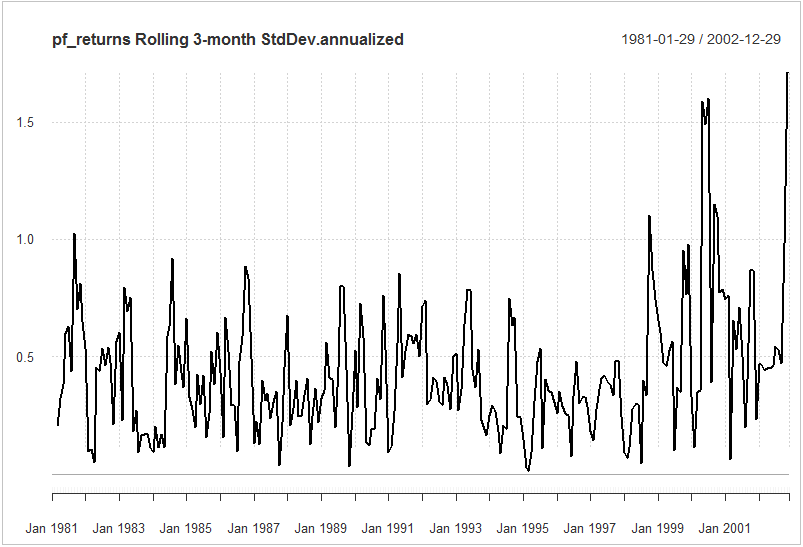
\includegraphics[scale=0.4]{sd_dynamics_pf_returns_3months_in_sample.PNG}
    \caption{Dynamics of Standard-Deviation of Portfolio Returns (In-Sample)}
    \end{center}
\end{figure}
\begin {figure}[H]
    \begin{center}
    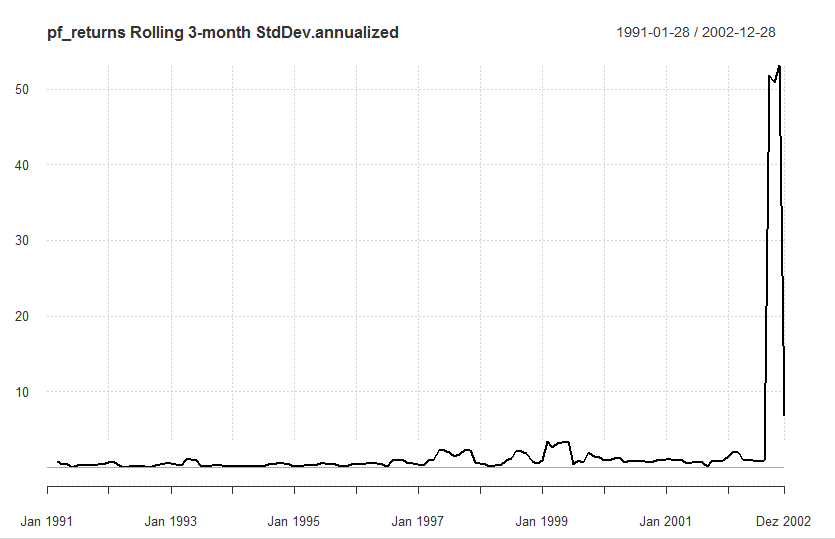
\includegraphics[scale=0.4]{sd_dynamics_pf_returns_3months_out_of_sample.PNG}
    \caption{Dynamics of Standard-Deviation of Portfolio Returns (Out-of-Sample)}
    \end{center}
\end{figure}
As shown in the graphs the dynamics of the out-of-sample SD are constant during most periods, whereas the in-sample SD varies during the whole observation period. This means that the in-sample returns are marked by a continuously changing volatility, which in turn implies unpredictability and a higher probability of an estimation error. By contrast, the out-of-sample returns' volatility is stable, which enables more accurate estimations and hence a more plausible long-term planning. In this context, it is essential to point out, that constant volatility should not be associated with higher portfolio returns, meaning that these two plots are only then an appropriate conclusion basis when the risk constancy is considered and not the portfolio's rentability. Thus, the graphs do not contain any final statements in terms of an investor's utility.  
\subsubsection{Dynamics of the Portfolio's Returns}
This subsection takes into account what section 3.2.1 does not, namely the rentability of an investor's portfolio. Figures 3 and 4 visualize the development of the portfolio's returns in- and out-of-sample.
\begin {figure}[htb]
    \begin{center}
    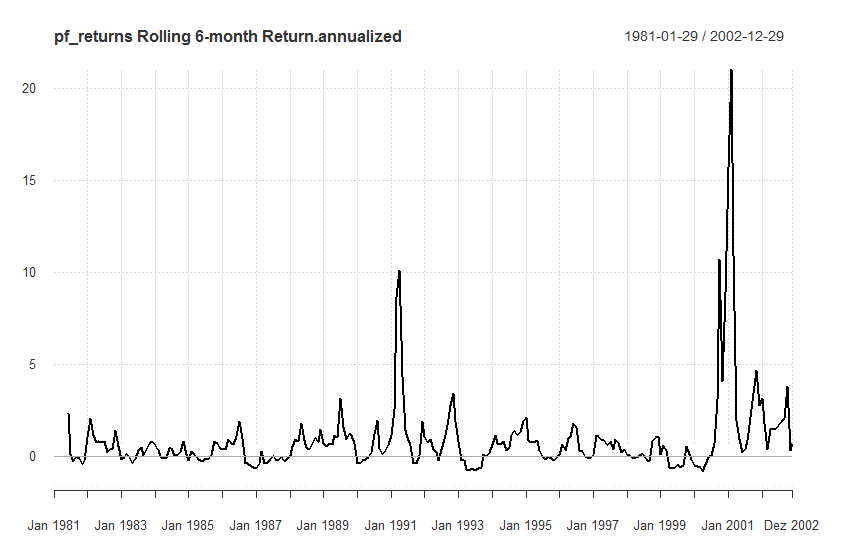
\includegraphics[scale=0.4]{portfolio_returns_dynamics_adjusted_in_sample.PNG}
    \caption{Dynamics of Portfolio Returns (In-Sample)}
    \end{center}
\end{figure}
\begin {figure}[H]
    \begin{center}
    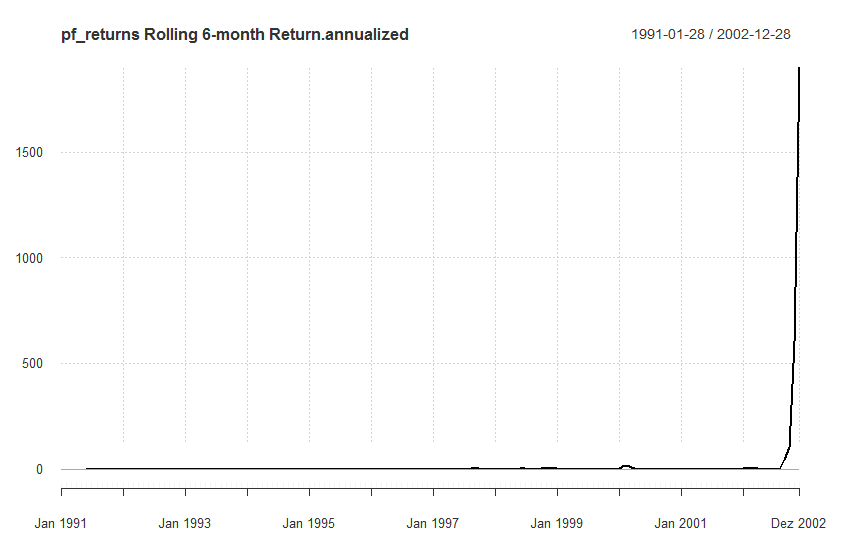
\includegraphics[scale=0.4]{portolio_returns_dynamics_adjusted_out_of_sample.PNG}
    \caption{Dynamics of Portfolio Returns (Out-of-Sample)}
    \end{center}
\end{figure}
The in-sample portfolio returns are in average higher than the out-of-sample ones. However, they also fluctuate stronger. Thus, the graph leads to the conclusion that the portfolio returns in-sample are higher and associated with a higher volatility. The out-of-sample plot over the same period barely shows any deviation, but very low average returns. As already discussed in section 3.1.1 a portfolio's performance should rather be evaluated out-of-sample. Consequently, an investor would take into consideration graph 4 and base his investment decision on it. Thus, Figure 3 could be misleading as it according to it the portfolio promises higher average returns in exchange for a higher (however relatively constant) risk. 
\subsubsection{Dynamics of relative Weights of Asset Returns}
Figures 5 and 6 visualize the way the relative weights change over time when the rolling window is set to 120. In this context, the relative weights of each asset fluctuate a lot more when the risk-free rate is not subtracted (Figure 5) compared to the ones of the excess asset returns (Figure 6). 
\begin {figure}[H]
    \begin{center}
    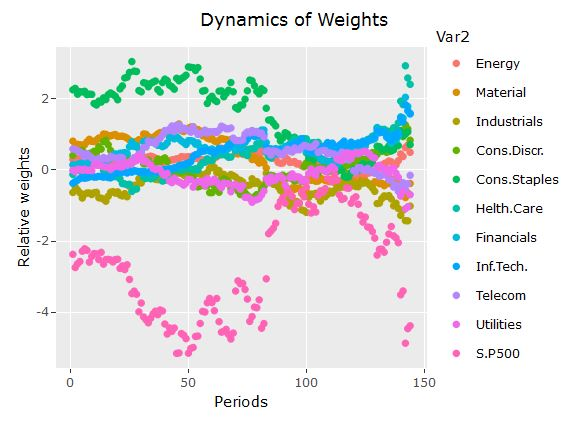
\includegraphics[scale=0.7]{dn_wg_unadj_MV.JPG}
    \caption{Dynamics of Weights (unadjusted Returns)}
    \end{center}
\end{figure}

\begin {figure}[H]
    \begin{center}
    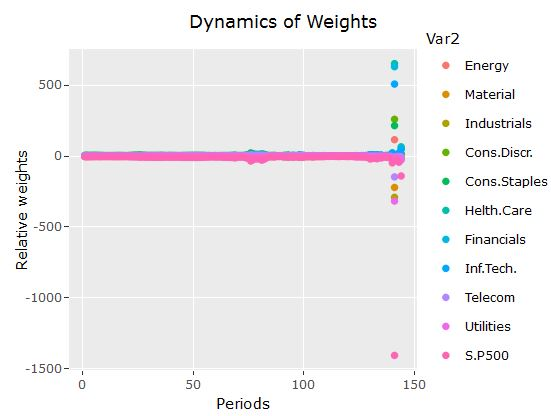
\includegraphics[scale=0.7]{dn_wg_adj_MV.JPG}
    \caption{Dynamics of Weights (Excess Returns)}
    \end{center}
\end{figure}\\
On the one hand, the unadjusted asset returns are higher than the excess ones. On the other hand, the higher values results into a higher fluctuation of the respective relative weights over time which also implies higher volatility as the investors would have to restructure their optimal portfolio in each period. This in turn leads to the inability to build a model that can be applied for long-term predictions. Therefore, risk adjustment has to be performed despite the fact that it results into asset returns whose values are reduced.
\subsubsection{Benchmark Comparison}
This section provides both a qualitative and a quantitative  comparison between the weighted portfolio's returns and the ones of the benchmark portfolio. Figures 7 and 9 visualize the in-sample and the out-of-sample comparison. Figures 8 and 10 quantify the graphs by computing the mean and the standard deviation of both portfolio's returns. 
\begin {figure}[H]
    \begin{center}
    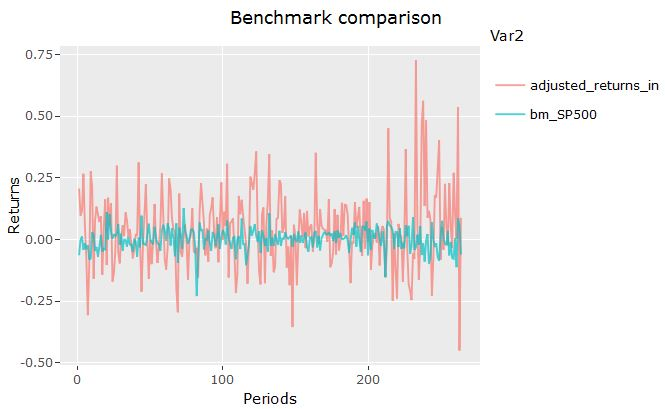
\includegraphics[scale=0.7]{Benchmark_in_sample_MV.JPG}
    \caption{Benchmark comparison in-sample}
    \end{center}
\end{figure}\\
\begin {figure}[H]
    \begin{center}
    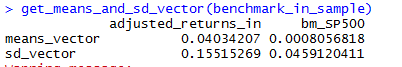
\includegraphics[scale=0.6]{benchmark_comparison_pf_returns_quantified_summary_in_sample.PNG}
    \caption{Benchmark comparison in-sample}
    \end{center}
\end{figure}\\
\begin {figure}[H]
    \begin{center}
    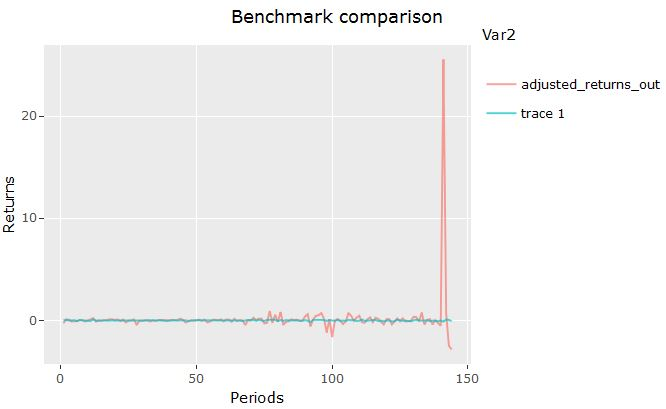
\includegraphics[scale=0.7]{Benchmark_out_of_sample_MV.JPG}
    \caption{Benchmark comparison out-of-sample}
    \end{center}
\end{figure}\\
\begin {figure}[H]
    \begin{center}
    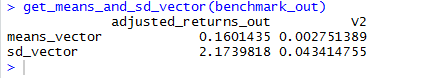
\includegraphics[scale=0.6]{benchmark_comparison_pf_returns_quantified_summary_out_of_sample.PNG}
    \caption{Benchmark comparison out-of-sample}
    \end{center}
\end{figure}\\
Like in all previous sections, the out-of-sample approach shows a lower risk and lower expected returns. In both cases the weighted portfolio has higher expected returns and higher volatility (measured by the standard deviation). The answer to the question which alternative an investor would choose is not clear, because the decision depends on the investor's utility function and their risk aversion. Each investor would choose opt for the investment which maximizes their utility.
\section{Conclusion}
This work provides a comparison between the mean-variance strategy and the Kan and Zhou three-fund portfolio strategy as a mixture of the minimum-variance strategy and the mean-variance strategy. Both alternatives were evaluated  according to their sharpe ratios and certainty equivalents in-sample and out-of-sample. The general statement of the work is that the mean-variance strategy performs slightly better than the three-fund portfolio strategy. The empirical results slightly deviate from the ones provided in DeMiguel et al. \cite{DEM09}. However, the general relations between the metrics are unchanged and the results remain plausible. The work leads to the conclusion that the investors should evaluate their investment out-of-sample, because an in-sample approach may be misleading. 
A possible extension of the current work consists in adding further evaluation metrics like a portfolio turnover. Furthermore, a basic benchmark strategy could also be considered and could serve as a reference point when evaluating the performance of the other strategies. In addition, to get a more extensive range of alternatives, further strategies could be considered, ranked under each other according to the evaluation metrics and compared to the benchmark strategy. Modifying each strategy by setting a short-sale constraint also widens the spectrum of possible investments. Besides, a plausibility check would be reasonable - one option would be to perform the analysis on various data sets containing the returns of different companies and referring to different benchmark portfolios/indexes. Moreover, a significance p-value test e.g. could be performed in order to determine whether the differences between the evaluation metrics are significant.      
\medskip
\medskip
\printbibliography
\appendix
\section{Code Appendix}
\begin{lstlisting}[caption={This listing shows the entire code developed in R.}, label=code:1,frame=single]
# set the working directory
setwd("C:\\Users/TO/Desktop")

# load the dataset
data=read.csv("ten-roberto-wessels.csv",sep=";",header=TRUE) 

# Install all necessary packages
install.packages("ggplot2")
install.packages("dygraphs")
install.packages("tidyverse")
install.packages("lubridate")
install.packages("zoo")
install.packages("xts")
install.packages("reshape2")
install.packages("plotly")
install.packages("PerformanceAnalytics")
install.packages("corrplot")
set.seed(123)
# Load the packages
library(ggplot2)
library(dygraphs)
library(tidyverse)
library(lubridate)
library(zoo)
library(xts)
library(reshape2)
library(plotly)
library(PerformanceAnalytics)
library(corrplot)

###################################################################
# STRATEGY-INDEPENDENT FUNCTIONS

# Function for calculating the means of every column/asset in the dataset:
get_means_vector=function(data){
  means_vector=apply(data,2,mean)
  return(means_vector)
}

# Function for calculating the SD of each column/asset in the dataset:
get_sd_vector=function(data){
  sd_vector=apply(data,2,sd)
  return(sd_vector)
}

# Function for calculating the relative weights of the assets in the dataset:
get_rel_weights_vector=function(weights_vector){
  
  # Calculate the absolute sum of the weights vector:
  abs_sum=abs(sum(weights_vector))

  # Divide each of the values in the absolute weights vector by the absolute sum:
  rel_weights=weights_vector/abs_sum

  #return the vector with the relative asset weights
  return (rel_weights)
}

# Function for getting the in-sample sharpe ratio OR the in-sample portfolio returns
get_insample_sharperatio_returns = function (data, absolute_weights_vector, sharperatio){
  
  # Create a new vector to be filled with the portfolio returns in sample in a loop rowise:
  pf_rtr_in_sample=c(length=length(data[,1]))
  for(i in 1:(length(data[,1]))){
    pf_rtr_in_sample[i]=unlist(data[i,])%*%(get_rel_weights_vector(absolute_weights_vector))
  }
  
  # an if-else construct to determine whether the in-sample sharpe ratio or the in-sample portfolio returns must be returned
  if (sharperatio == TRUE) { # compute the sharpe ratio in-sample applying the formula from DeMiguel page 1928
    return (mean(pf_rtr_in_sample)/sd(pf_rtr_in_sample)) 
  } else { # return the portfolio returns in-sample
    return (pf_rtr_in_sample)
  }
}

# Function for getting the out-of-sample sharpe ratio OR the out-of-sample portfolio returns
get_outofsample_sharperatio_returns = function (M, data, sharperatio, strategy) {
  
  # set the rolling window:
  rolling_window=M
  
  # Calculate length of the new vector with the portfolio returns:
  len_portfolio_returns=length(data[,1])-rolling_window
  
  # Create the vector with the respective length:
  portfolio_returns_outofsample=c(length=len_portfolio_returns)
  
  # Calculate the (in this case 264 - 120) excess returns and add each value in the portfolio_returns vector:
  for(i in 1:len_portfolio_returns){
    # Set the start index for each iteration:
    start_window=i
    
    # Set the start index for each iteration:
    end_window=rolling_window+i-1
    
    # Create a new "time"-matrix, which contains the data for a certain 120-days period
    # with the start index and the end index (rowise):
    time_matrix=data[start_window:end_window,]
    
    # Create the covariance matrix of the "time"-matrix:
    cov_time_matrix=cov(time_matrix)
    
    # Calculate the absolute weights of the assets in row end_window + 1 based on the last 120 rows:
    # an if-else construct to differentiate between both strategies, since these require different functions 
    if (strategy == "mv") { # mean-variance strategy
      weights_vct=get_weights_vector(get_means_vector(time_matrix),cov_time_matrix)
    } else { # Kan and Zhou three-fund portfolio strategy
      weights_vct=get_weights(time_matrix, length(time_matrix[,1]), length(time_matrix[1,]))
    }
    
    # Calculate the portfolio return using the excess returns in row 
    # end_window + 1 of the initial data and the computed relative weights:
    single_pf_return=unlist(data[end_window+1,])%*%get_rel_weights_vector(weights_vct)
    
    # Add each value in the vector portfolio returns:
    portfolio_returns_outofsample[start_window]=single_pf_return
  }
  
  portfolio_returns_outofsample = c(t(portfolio_returns_outofsample))
  
  # an if-else construct to determine whether the out-of-sample sharpe ratio or the out-of-sample portfolio returns must be returned
  if (sharperatio == TRUE) { # compute the out-of-sample sharperatio
    sharpe_ratio_out_of_sample=mean(portfolio_returns_outofsample)/sd(portfolio_returns_outofsample)
    return (sharpe_ratio_out_of_sample) 
  } else { # return the out-of-sample portfolio returns
    return (portfolio_returns_outofsample)
  }
}

# Function for calculating the dynamics of weights all of the T-M periods (T = total observations, M = rolling window)  

# description of the function's parameters
# 1. M: a numeric variable ->length of the rolling window
# 2. data: a data frame -> the relevant data 
# 3. assets: a numeric variable -> amount of assets considered
# 4. cov_matrix: a boolean variable -> the cov_matrix needed to compute the absolute weights vector for the mean-variance strategy;
#    the Khan and Zou strategy doesn't require a cov-matrix for the computation of the absolute weights vector
#    => if assigned TRUE, the function computes the absolute weights vector according to the mean-variance strategy
#       if assigned FALSE, the function computes the absolute weights vector according to the Kan and Zhou strategy


get_weights_dynamics = function(M, data, assets, cov_matrix) {
  
  # create an empty matrix which should collect the relative weights vector for each period considered
  collector = matrix(, nrow = assets, ncol = (length(data[,1])-M))
  colnames(collector) = c(1:(length(data[,1])-M))
  rownames(collector) = c(colnames(data))
  
  for(i in 1:(length(data[,1])-M)) {
    # Set the start index for each iteration:
    start_window=i
    
    # Set the start index for each iteration:
    end_window=M+i-1
    
    # Create a new "time"-matrix with the start index and the end index (rowise) to collect the absolute r.w. difference in t:
    time_matrix=data[start_window:end_window,]
    
    # an if-else construct to distinguish between the mean-variance and the Khan and Zou strategy, since the computation of
    # the abssolute weights vectors are different for both strategies
    
    if (cov_matrix == TRUE) { # mean-variance strategy
      # Create the covariance matrix of the time matrix
      cov_time_matrix=cov(time_matrix)
      # Calculate the absolute weights of the assets over time (always based on the previous 120 rows)
      weights_vct=get_weights_vector(get_means_vector(time_matrix), cov_time_matrix)
    } else { # Khan and Zou three-fund portfolio strategy
      weights_vct=get_weights(time_matrix, M, assets)
    }
    # Calculate the relative weights (the function for the computation of the relative weights is not strategy-dependent)
    rel_weights_vct=get_rel_weights_vector(weights_vct)
    
    # Collect the relative weights vectors for each period in the collector-matrix
    collector[,i] = rel_weights_vct
  }
  
  # transpose the collector matrix
  weight_matrix = t(collector)
  
  # plot a basic ggplot
  p1= ggplot(melt(weight_matrix), aes(x=Var1, y=value, col=Var2))+geom_point()+ggtitle("Dynamics of Weights")+ylab("Relative weights")+xlab("Periods")
  # make the basic ggplot interactive
  dynamics_return = ggplotly(p1)
  
  return(dynamics_return)
}

# Function for plotting the SD dynamics OR the development of a portfolio's returns over time

# description of the function's parameters
# 1. portfolio_returns: a data frame or a matrix, containing the in-sample or out of sample portfolio returns over time
# 2. width: the interval (2 months, 6 months, 1 year etc.), over which the function should be applied -> in months!
# 3. SD: a boolean variable 
#    => if assigned TRUE, the function plots the SD dynamics
#    => if assigned FALSE, the function plots the portfolio's returns dynamics

get_sd_dynamics_or_devreturn = function(portfolio_returns, width, sd, dates_seq) {
  
  pf_returns = portfolio_returns
  pf_returns = data.frame(pf_returns)
  
  # assign the sequence the rows of the return's data frame
  rownames(pf_returns)=dates_seq
  
  # format the data frame as time series
  pf_returns=as.xts(pf_returns,dateFormat="Date")
  
  #an if-else construct to differentiate which function should be applied
  if (sd == TRUE) { #plot the SD dynamics
    b = chart.RollingPerformance(R = pf_returns, width = width, FUN = "StdDev.annualized")
  } else { # plot the portfolio returns' dynamics
    b = chart.RollingPerformance(R = pf_returns, width = width, FUN = "Return.annualized")
  }
  return(b)
}

# Function for making a benchmark comparison: plot the development of the weighted portfolio's returns versus the returns
# of the benchmark portfolio

# hand over a benchmark matrix or data frame, which contains the weighted portfolio's returns and the returnss of the 
# benchmark portfolio over time
bm_comparison = function (benchmark) {
  
  bm_df = data.frame(benchmark)
  
  #turn the benchmark object into a matrix with appropriate length, width and names
  bm_mat = matrix(benchmark, nrow = (length(bm_df[,1])), ncol = (length(bm_df[1,])))
  rownames(bm_mat) = c(1:(length(bm_df[,1])))
  colnames(bm_mat) = c(colnames(benchmark))
  
  #plot a basic ggplot
  bm= ggplot(melt(bm_mat), aes(x=Var1, y=value, col=Var2))+geom_line(alpha = 0.7)+ggtitle("Benchmark comparison")+ylab("Returns")+xlab("Periods")
  
  
  #make the basic ggplot interactive
  plot = ggplotly(bm)
  
  return(plot)
}

# Function for getting the means and sd vector of the data frame from the function above
# hand over the same parameter as in the function above
get_means_and_sd_vector = function(benchmark_c) {
  
  df = data.frame(benchmark_c)
  # compute the means vector of the weighted portfolio's returns and the benchmark returns 
  bm_means = get_means_vector(df)
  
  # compute the SD vector of the weighted portfolio's returns and the benchmark returns
  bm_sd = get_sd_vector(df)
  
  # create an empty matrix with an appropriate length, width and names
  sum_matrix = matrix(, nrow = length(bm_means), ncol = 2)
  rownames(sum_matrix) = c(colnames(df))
  colnames(sum_matrix) = c("means_vector", "sd_vector")
  
  # fill the matrix with the computed vectors
  sum_matrix[,1] = bm_means
  sum_matrix[,2] = bm_sd
  
  # return the transposed matrix
  return(t(sum_matrix))
  
}

###################################################################
# MEAN VARIANCE STRATEGY SPECIFIC FUNCTIONS

# Function for calculating the absolute weights of the assets in the dataset:
get_weights_vector= function(means_vector,cov_matrix){
  
  # Create the inverse of the passed covariance matrix:
  inverse_cov=solve(cov_matrix)
  
  # Implement the formula for Xt (DeMiguel, Garlappi, Uppal; page 1922):
  x_t=inverse_cov%*%means_vector
  x_t_vector=c(x_t)
  
  # return the vector with the absolute asset weights
  return (x_t_vector)
}


###################################################################
# KAN AND ZHOU THREE FUND STRATEGY PORTFOLIO SPECIFIC FUNCTIONS

# Function for getting the mu-g-parameter from the Kan and Zhou paper page 643
# by dimensions is meant the amout of assets in the dataset
get_mu_g = function(data, dimensions){
  
  # compute the inverse matrix of the covariance matrix of the data
  inverse_matrix = solve(cov(data))
  
  # create a n-dimensional 1-vector
  vec1 = numeric(0)
  i_vector = c(vec1, 1:dimensions)
  i_vector[1:dimensions] = 1
  
  # compute the nominator and the denominator needed for the final division
  nominator =  (t(get_means_vector(data))) %*%inverse_matrix%*%i_vector
  denominator = (t(i_vector)) %*%inverse_matrix%*%i_vector
  
  # get mu_g and make it a vector
  mu_g = nominator/denominator
  mu_g = as.vector(mu_g)
  
  return (mu_g)
}

# Function for computing the psi^2-parameter from the Kan and Zhou paper page 643
get_psi_square = function(data, mu_g_object, dimensions ){
  
  # compute the inverse matrix of the covariance matrix of the data
  inverse_matrix = solve(cov(data))
  
  # create a n-dimensional 1-vector
  vec1 = numeric(0)
  i_vector = c(vec1, 1:dimensions)
  i_vector[1:dimensions] = 1
  
  # get psi^2 and make it a vector
  psi_square = (t(get_means_vector(data)) - mu_g_object*i_vector) %*% inverse_matrix %*% (get_means_vector(data) - mu_g_object*i_vector)
  psi_square = as.vector(psi_square)
  
  return (psi_square)
}

# Function for computing the c3-parameter from the Kan and Zhou paper page 636
get_c3 = function(observations, dimensions){
  
  # get the first and the second term for the final multiplication
  first_term = (observations-dimensions-4)/observations
  second_term = (observations-dimensions-1)/(observations-2)
  
  # get the c3-parameter
  c3 = first_term*second_term
  
  return(c3)
}

# Function for computing the absolute weights vector of a Kan and Zhou three fund portfolio from the Kan and Zhou paper page 642
get_weights = function(data, observations, dimensions) {
  
  # get the c3 paremeter
  c3_object = get_c3(observations, dimensions)
  
  # get the mu_g parameter
  mu_g_object =get_mu_g(data, dimensions)
  
  # get the psi^2 parameter
  psi_square_object = get_psi_square(data, mu_g_object, dimensions)
  
  # compute the inverse matrix of the covariance matrix of the data
  inverse_matrix = solve(cov(data))
  
  # create a n-dimensional 1-vector
  ma = matrix(1, 1, dimensions) 
  i_vector = c(ma)
  
  # get the means vector of the data
  means_vector = get_means_vector(data)
  
  # compute the first and the second term for the final multiplication
  first_term = (psi_square_object/(psi_square_object+(dimensions/observations))) * inverse_matrix %*%means_vector
  second_term = ((dimensions/observations) / (psi_square_object + (dimensions/observations))) * mu_g_object * inverse_matrix %*% i_vector
  
  # get the absolute weights vector
  weights = c3_object * (first_term + second_term)
  
  return(weights)
}

###################################################################
#0) Subsetting and predefinition of constants

# a subset without the date-column
data.red=data[,-1]

# a subset, containing the excess returns (after subtracting the risk-free rate in column for each period -> column 13 in the original dataset)
# the return in the initial dataset still contain a risk free rate 
#data.new=data.red[,-12]-data.red[,12]
data.new=matrix(,nrow=264, ncol=11)
colnames(data.new)=c(colnames(data[,2:12]))
for (i in 1:11){
  data.new[,i]=data.red[,i]-data.red[,12]
}
data.new=data.frame(data.new)


# create a subset, containing the non-excessive returns (the original data)
data.probe = data.red[,-12]

# create a subset, containing the benchmark SP500-portfolio
bm_SP500 = data.new$S.P500

# determine the amount of assets considered
assets = length(data.new[1,])

# determine the amount of observations considered
observations = length(data[,1])

###################################################################
# APPLYING THE FUNCTIONS TO THE MEAN VARIANCE STRATEGY

#1) Calculate the Sharpe ratio -> excess returns needed => use the data.new subset

#1.1) out-of-sample

sharpe_ratio_out_of_sample_mv=get_outofsample_sharperatio_returns(120, data.new, TRUE, "mv")
round(sharpe_ratio_out_of_sample_mv, digits=4)
#1.2) in-sample

# 1. alternative
sharpe_ratio_in_sample_mv=get_insample_sharperatio_returns(data.new, get_weights_vector((get_means_vector(data.new)), cov(data.new)), TRUE)
round(sharpe_ratio_in_sample_mv, digits=4)
# 2. alternative: apply the integrated SharpeRatio-function in R as a check
dates=seq(as.Date("1981/01/30"), as.Date("2002/12/31"), by = "1 month",tzone="GMT")-1
rownames(data.new)=dates
time_series=as.xts(data.new,dateFormat="Date")

# compute the relative weights vector: needed for the weights-parameter of the integrated SharpeRatio function in R
aw = get_weights_vector((get_means_vector(data.new)), cov(data.new)) # absolute
rw = get_rel_weights_vector(aw) # relative
SharpeRatio(R = time_series, Rf = 0, p = 0.95, FUN = c("StdDev"),weights = rw, annualize = FALSE)

#3) calculate the certainty-equivalent -> unadjusted returns needed => use the data.probe subset

#3.1) out-of-sample 

# compute the out-of-sample portfolio returns
returns_out= get_outofsample_sharperatio_returns(120, data.probe, FALSE, "mv")

# compute the out-of-sample certainty-equivalent:
certainty_equivalent_out_of_sample_mv=mean(returns_out) - ((1/2)*(var(returns_out)))
round(certainty_equivalent_out_of_sample_mv,digits=4)
#3.2) in-sample

# compute the absolute weights vector of the returns: needed as a parameter for the following function
absolute_weights_in = get_weights_vector((get_means_vector(data.probe)), cov(data.probe))

# compute the in-sample portfolio returns
returns_in = get_insample_sharperatio_returns(data.probe, absolute_weights_in, FALSE )

certainty_equivalent_in_sample_mv=mean(returns_in) - (1/2)*(var(returns_in))
round(certainty_equivalent_in_sample_mv,digits=4)
#4) Plotting the dynamics of a portfolio returns' SD: the plot is based on a 3-month interval 
#   adjusted returns => data.new subset

#4.1) in-sample portfolio returns

# compute the absolute weights vector of the adjusted returns: needed as a parameter for the following function
absolute_weights_adj = get_weights_vector((get_means_vector(data.new)), cov(data.new))

# compute the adjusted in-sample adjusted portfolio returns 
adjusted_returns_in = get_insample_sharperatio_returns(data.new, absolute_weights_adj, FALSE )

# create a sequence of the dates of the observations: needed as a parameter for the following function
dates_in=seq(as.Date("1981/01/30"), as.Date("2002/12/31"), by = "1 month",tzone="GMT")-1

# plot SD dynamics of the in-sample portfolio returns
get_sd_dynamics_or_devreturn(adjusted_returns_in, 3, TRUE, dates_in)

#4.2) out-of-sample portfolio returns

# compute the adjusted out-of-sample adjusted portfolio returns
adjusted_returns_out = get_outofsample_sharperatio_returns(120, data.new, FALSE, "mv")

# create a sequence of the dates of the observations: needed as a parameter for the following function
data.new[121,]
data.new[264,]
dates_out=seq(as.Date("1991/01/29"), as.Date("2002/12/29"), by = "1 month",tzone="GMT")-1

# plot SD dynamics of the out-of-sample portfolio returns
get_sd_dynamics_or_devreturn(adjusted_returns_out, 3, TRUE, dates_out)

#6) Plotting the dynamics of weights of all assets

# based on unadjusted portfolio returns
get_weights_dynamics(120, data.probe, 11, TRUE)

# based on adjusted portfolio returns
get_weights_dynamics(120, data.new, 11, TRUE)

#7) Plotting the dynamics of a portfolio's returns: the plot is based on a 6-month interval

# based on unadjusted in-sample portfolio returns
get_sd_dynamics_or_devreturn(returns_in, 6, FALSE, dates_in)

# based on unadjusted out-of-sample portfolio returns
get_sd_dynamics_or_devreturn(returns_out, 6, FALSE, dates_out)

# based on adjusted in-sample portfolio returns
get_sd_dynamics_or_devreturn(adjusted_returns_in, 6, FALSE, dates_in)

# based on adjusted out-of-sample portfolio returns
get_sd_dynamics_or_devreturn(adjusted_returns_out, 6, FALSE, dates_out)

#8) Benchmark comparison in sample 

benchmark_in_sample = cbind(adjusted_returns_in, bm_SP500)

bm_comparison(benchmark_in_sample)
get_means_and_sd_vector(benchmark_in_sample)

#9) benchmark comparison out of sample 

W = 120 + 1
L = length(data[,1])
benchmark_out = cbind(adjusted_returns_out, bm_SP500[W:L])

bm_comparison(benchmark_out)
get_means_and_sd_vector(benchmark_out)

###################################################################
# APPLYING THE FUNCTIONS TO THE KAN AND ZHOU THREE FUND PORTFOLIO STRATEGY


#1) Calculate the Sharpe ratio -> excessive returns needed => use the data.new subset

#1.1) out-of-sample

sharpe_ratio_out_of_sample_kz=get_outofsample_sharperatio_returns(120, data.new, TRUE, "kz")
round(sharpe_ratio_out_of_sample_kz, digits=4)
#1.2) in-sample

# 1. alternative
sharpe_ratio_in_sample_kz=get_insample_sharperatio_returns(data.new, get_weights(data.new, observations, assets), TRUE)
round(sharpe_ratio_in_sample_kz, digits=4)

# 2. alternative: apply the integrated SharpeRatio-function in R as a check
dates_kz=seq(as.Date("1981/01/30"), as.Date("2002/12/31"), by = "1 month",tzone="GMT")-1
rownames(data.new)=dates_kz
time_series_kz=as.xts(data.new,dateFormat="Date")

# compute the relative weights vector: needed for the weights-parameter of the integrated SharpeRatio function in R
aw_kz = as.vector(get_weights(data.new, observations, assets)) # absolute
rw_kz = get_rel_weights_vector(aw_kz) # relative
SharpeRatio(R = time_series_kz, Rf = 0, p = 0.95, FUN = c("StdDev"),weights = rw_kz, annualize = FALSE)

#3) calculate the certainty-equivalent -> unadjusted returns needed => use the data.probe subset

#3.1) out-of-sample (passt)

# compute the out-of-sample portfolio returns
returns_out_kz= get_outofsample_sharperatio_returns(120, data.probe, FALSE, "kz")

# compute the out-of-sample sharpe ratio
certainty_equivalent_out_of_sample_kz=mean(returns_out_kz) - ((1/2)*(var(returns_out_kz)))
round(certainty_equivalent_out_of_sample_kz,digits=4)
#3.2) in-sample

# compute the absolute weights vector of the returns: needed as a parameter for the following function
absolute_weights_kz = get_weights(data.probe, observations, assets)

# compute the in-sample portfolio returns
returns_in_kz = get_insample_sharperatio_returns(data.probe, absolute_weights_kz, FALSE )

certainty_equivalent_in_sample_kz=mean(returns_in_kz) - (1/2)*(var(returns_in_kz))
round(certainty_equivalent_in_sample_kz,digits=4)
#4) Plotting the dynamics of a portfolio returns' SD: the plot is based on a 3-month interval 
#   adjusted returns => data.new subset

#4.1) in-sample portfolio returns

# compute the absolute weights vector of the adjusted returns: needed as a parameter for the following function
absolute_weights_adj_kz = get_weights(data.new, observations, assets)

# compute the adjusted in-sample adjusted portfolio returns 
adjusted_returns_in_kz = get_insample_sharperatio_returns(data.new, absolute_weights_adj_kz, FALSE )

# create a sequence of the dates of the observations: needed as a parameter for the following function
dates_in_kz=seq(as.Date("1981/01/30"), as.Date("2002/12/31"), by = "1 month",tzone="GMT")-1

# plot SD dynamics of the in-sample portfolio returns
get_sd_dynamics_or_devreturn(adjusted_returns_in_kz, 3, TRUE, dates_in_kz)

#4.2) out-of-sample portfolio returns

# compute the adjusted out-of-sample adjusted portfolio returns
adjusted_returns_out_kz = get_outofsample_sharperatio_returns(120, data.new, FALSE, "kz")

# create a sequence of the dates of the observations: needed as a parameter for the following function
data.new[121,]
data.new[264,]
dates_out_kz=seq(as.Date("1991/01/29"), as.Date("2002/12/29"), by = "1 month",tzone="GMT")-1

# plot SD dynamics of the out-of-sample portfolio returns
get_sd_dynamics_or_devreturn(adjusted_returns_out_kz, 3, TRUE, dates_out_kz)

#6) Plotting the dynamics of weights of all assets

# based on unadjusted portfolio returns
get_weights_dynamics(120, data.probe, 11, FALSE)

# based on adjusted portfolio returns
get_weights_dynamics(120, data.new, 11, FALSE)

#7) Plotting the dynamics of a portfolio's returns: the plot is based on a 6-month interval

# based on unadjusted in-sample portfolio returns
get_sd_dynamics_or_devreturn(returns_in_kz, 6, FALSE, dates_in_kz)

# based on unadjusted out-of-sample portfolio returns
get_sd_dynamics_or_devreturn(returns_out_kz, 6, FALSE, dates_out_kz)

# based on adjusted in-sample portfolio returns
get_sd_dynamics_or_devreturn(adjusted_returns_in_kz, 6, FALSE, dates_in_kz)

# based on adjusted out-of-sample portfolio returns
get_sd_dynamics_or_devreturn(adjusted_returns_out_kz, 6, FALSE, dates_out_kz)

#8) Benchmark comparison in sample 

benchmark_in_sample_kz = cbind(adjusted_returns_in_kz, bm_SP500)

bm_comparison(benchmark_in_sample_kz)
get_means_and_sd_vector(benchmark_in_sample_kz)

#9) benchmark comparison out of sample 

W = 120 + 1
L = length(data[,1])
benchmark_out_kz = cbind(adjusted_returns_out_kz, bm_SP500[W:L])

bm_comparison(benchmark_out_kz)
get_means_and_sd_vector(benchmark_out_kz)

#10) correlation matrix of the 11 assets + the one benchmark 

corr_matrix = cor(data.new)
corrplot(corr_matrix, method="number", number.cex = 0.5)

\end{lstlisting}


\end{document}
